\section{(Alternate) Predicting ELMS in sequences using the API}
\label{sec:predicting_REST}

Querying ELM for motifs in a given sequence (as discussed in basic
protocol 1), gives you a nice overview of putative and possibly
annotated motifs in your query protein with a graphical representation
using colors to highlight different regions of the protein sequence (eg.
disordered vs.~globular). It is however difficult to analyse a large set
of protein sequences in this manner. Therefore, http://elm.eu.org
provides an interface which you can use to submit your sequence in a
programmatic way. Of course, this way, you won't receive the graphical
output representation, but are limited to textual data representation.

Currently, there exists a single URL `http://elm.eu.org/start\_search/'
to accept such queries. You can choose to either submit a uniprot name
or accession (ex. `http://elm.eu.org/start\_search/P53\_HUMAN.tsv') or
submit your raw sequence (ex.
`http://elm.eu.org/start\_search/MAPRGFSCLLLLTSEIDLPVKRRA').

The logic here is, if the URL ends in `.tsv' then the server assumes you
are using a Uniprot id or accession; if it doesn't, then it assumes you
are using raw sequence. See below for details.

%
% Subsection: Necessary Resources
%
\subsection{Necessary Resources}

\subsubsection{Software}

Ideally use \texttt{curl} https://curl.haxx.se/ on the command line.
This program can be launched from the terminal in any of the major
operating systems: OSX, Windows and Linux. Of course \texttt{curl} is
only one of many different ways to access web content programatically,
and we suggest anyone to use which ever program they feel is better
suited for their tasks.

\begin{enumerate}

%
% Subsection: Submitting a query via the REST API
%
\subsection{Submitting a query to ELM via the REST API}
\label{subsec:predicting_REST_submitting}

\item Use \texttt{curl} to query ELM for all motifs predicted to occur in Human
	P53 by typing the following into a terminal: `curl
	`http://elm.eu.org/start\_search/P53\_HUMAN.tsv'. Each row represents a
	motif detection, and the first column ``elm\_identifier'' indicates
	which class was identified. The columns ``start'' and ``stop'' show
	that first and last amino acid positions that matched form part of the
	motif.  ``is annotated'' is True if this motif has been annotated in
	the database as an (experimentally validate) motif instance. ``is
	phiblastmatch'' is True if ?????. The column ``is filtered'' shows
	whether or not this motif was rejected by the ELM Prediction structure
	filter. ``phibast'' indicates whether ?????. The ``topodomfilter'' and
	``taxonfilter'' shown whether ?????. The last column ``structure''
	?????

	\sdesc{In Figure \emph{ELM predictions pP53} we used a sligtly more
		advanced command to get the output to look nice in the
		terminal. We specified the \texttt{-s} option to silence all
		\texttt{curl} output other than the downloaded file, and piped
		(\texttt{\textbar{}}) the output directly to the
		\texttt{column} command (this command exists on most Linux and
		OSX machines).}

TODO: REDO FIGURE as it shows browser in transparent background

\begin{figure}[h!]
	\centering
	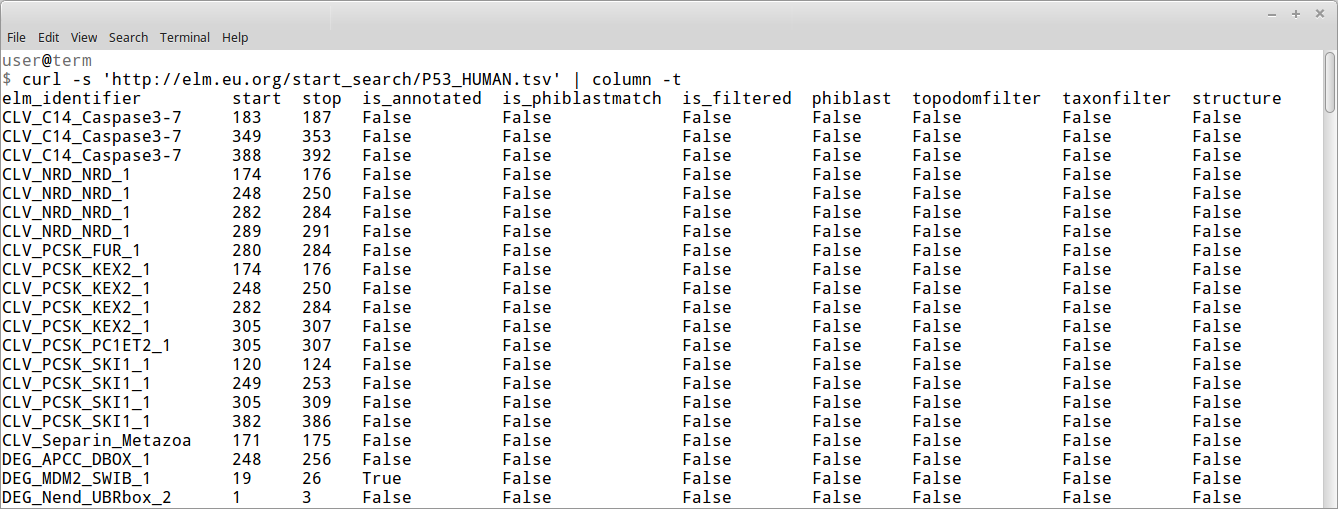
\includegraphics[width=\textwidth]{Figures/predicting_REST/curl_P53.png}
	\caption{
	\textbf{Figure ELM Predictions P53:}
	The commandline output when \texttt{curl} is used to
	donload all motifs predicted in Human P53. Note that we used a more
	advanced command that \texttt{curl} alone to make the columns align
	nicely (see text for an explanation).
	}
\end{figure}

\item Use \texttt{curl} to query ELM via protein sequence by using the URL
	`http://elm.eu.org/start\_search/MAPRGFSCLLLLTSEIDLPVKRRA' (Figure
	BACT-AP3-query). In this case the the query is an arbitrary short
	peptide sequence, but this can (of course) contain any sequence you are
	intersted in analysing. The output format is exactly the same as in the
	previous step.

	\sdesc{ This way of querying ELM is unfornataly not stable for long
		protein sequences. Different browsers and computers have
		different maximum lengths for URLs, and the excess text is
		often simply ignored. We reccomend not using this method for
		sequences longer than 2000 amino acids.}

TODO: REDO FIGURE as it shows browser in transparent background

\begin{figure}[h!]
	\centering
	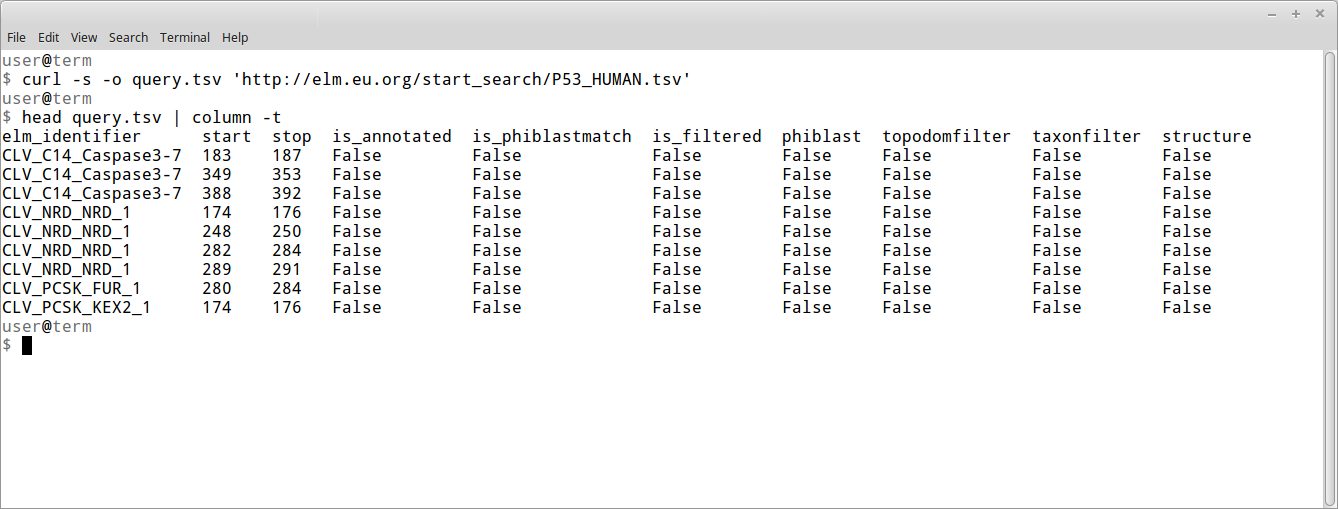
\includegraphics[width=\textwidth]{Figures/predicting_REST/predictions_query.png} 
	\caption{
	\textbf{Figure ELM Predictions on query sequence:}
	It is also possible to send amino
	acid sequences to the ELM Prediction pipeline. In this case we have used
	the curl option \texttt{-o} to download directly to the file
	\texttt{query.tsv}, and use a combination of the \texttt{head} and
	\texttt{column} commands to display the first 10 rows to the terminal.
	}
	\label{fig:predicting_REST_query}
\end{figure}

TODO: add this information to the download page

TODO: maybe rename \texttt{start\_search} to \texttt{query}?

\end{enumerate}
